%!TEX root = ./main.tex
\documentclass[12pt,letterpaper]{scrartcl}
\usepackage[secthm,mdthm,simplethm]{beel}
%!TEX root = ./main.tex
\usepackage{graphicx}
\usepackage{tcolorbox}
\usepackage[margin=1in,top=0.8in, bottom = 0.8in]{geometry}
%%%%%%Packages%%%%%%%%%%%%%
\usepackage{amsmath}
\usepackage{amsfonts}
\usepackage{amsthm}
\usepackage{amssymb}
\usepackage{array}
\usepackage{comment}
\usepackage{enumitem}
\usepackage{graphicx}
\usepackage{hyperref}
\usepackage[utf8]{inputenc}
\usepackage{mathtools}
\usepackage{multicol}
\usepackage{tabto}
\usepackage{tikz}
\usepackage{pgfplots}
\usepackage{setspace}
\usepackage[all]{xy}
\usepackage{thmtools}
\usepackage{MnSymbol,wasysym}
\usepackage{venndiagram}
\usepackage{listings}
\usetikzlibrary{decorations.pathmorphing,shapes}
%%%%Theorem Enviorment Setup%%%%%%%
\begin{comment}
\theoremstyle{definition}
\newtheorem{theorem}{Theorem}[section]
\newtheorem{corollary}{Corollary}[theorem]
\newtheorem{lemma}[theorem]{Lemma}
\newtheorem{claim}[theorem]{Claim}
\newtheorem{definition}{Definition}[section]
\newtheorem{example}{Example}[section]
\newtheorem{remark}{Remark}[section]
\newtheorem{proposition}[theorem]{Proposition}
\end{comment}
\pgfplotsset{compat = 1.15}
%%%%%%%%%HyperLink Setup%%%%%%%%%%%
%
%%%%%%%%%%%%%%%Commands%%%%%%%%%%%%%%%%
\newcommand{\pml}{\begin{pmatrix}}
\newcommand{\pmr}{\end{pmatrix}}
\newcommand{\bml}{\left[ \begin{array}{ccccccccccccccccccccccccccccccccccccccccccccccccccccccccccc}}
\newcommand{\bmr}{\end{array} \right]}
\newcommand{\aml}{\left[ \begin{array}{rrr|r}}
\newcommand{\amr}{\end{array} \right]}
\newcommand{\vml}{\left\vert \begin{array}{rrrrrrrrrr}}
\newcommand{\vmr}{\end{array} \right\vert}
\renewcommand{\tab}{\hspace{1cm}}
\renewcommand{\b}{\mathbb}
\renewcommand{\c}{\mathcal}
\newcommand{\lb}{\left\{}
\newcommand{\rb}{\right\}}
\newcommand{\la}{\langle}
\newcommand{\ra}{\rangle}
\renewcommand{\bar}{\overline}
\newcommand{\ngroup}{\trianglelefteq}
\newcommand{\ver}{ \ | \ }
\renewcommand{\t}{\text}
\newcommand{\z}{\mathbb Z}
\renewcommand{\r}{\mathbb R}
\newcommand{\q}{\mathbb Q}
\newcommand{\ex}{\textbf{Example. }}
\renewcommand{\mod}[1]{\t{ (mod } {#1})}
\newcommand{\zz}[1]{\b Z/ {#1} \b Z}
\newcommand{\cg}[1]{\la {#1} \ra}
\newcommand{\li}[2]{{#1}_1,{#1}_2, \ldots, {#1}_{#2} }

% derivatives
\newcommand{\pd}[2]{\frac{\partial}{\partial #2} #1}
\newcommand{\dr}[2]{\frac{d}{d #2} #1}

% argmin/max
\DeclareMathOperator*{\argmax}{arg\,max}
\DeclareMathOperator*{\argmin}{arg\,min}

% matrix
\newcommand{\exh}[2]{{#1}_1\\{#1}_2\\\cdots\\{#1}_n}
\newcommand{\exv}[2]{{#1}_1\\{#1}_2\\\vdots\\{#1}_n}
\newcommand{\m}[1]{\begin{bmatrix}{#1}\end{bmatrix}}

\renewcommand{\v}{\vec}
% \renewcommand{\t}{\tilde}
\newcommand{\spa}{\text{span}}
\newcommand{\lincomb}[3]{{#1}_1{#2}_1 + {#1}_2{#2}_2 + \cdots + {#1}_{#3}{#2}_{#3}}
\newcommand{\nul}{\text{Null }}
\newcommand{\col}{\text{Col }}
\newcommand{\range}{\text{Range }}
\newcommand{\itab}{\hspace{-0.25cm}}
\newcommand{\omicron}{o}
\renewcommand{\qedsymbol}{$\blacksquare$}
% \renewcommand{\vec}{\mathbf}
\renewcommand{\Re}{\textrm{Re}}
\renewcommand{\Im}{\textrm{Im}}
%%%%%%%%%%%% main doc%%%%%%%%%%%%
\begin{document}
\thispagestyle{empty}
$ $
\vfill
\begin{center}
\centerline{\huge \textbf{EECS 127/227A, Fall 2022}}
\[
\]
\centerline{\huge \textbf{Optimization Models in Engineering}}
\[
\]
\centerline{\huge \text{Gireeja Ranade, UC Berkeley}}
\centerline{\huge \text{Zhiyu An}} 
\end{center}
\vfill
$ $
\newpage
\tableofcontents
\newpage
\renewcommand\thesubsection{\thesection.\alph{subsection}}
\renewcommand\thesubsubsection{\thesection.\roman{subsubsection}}
\section{Linear Algebra}

\subsection{Least-Squares Problem Statement} % (fold)
\label{sub:least_squares_problem_statement}

\begin{definition}[Least Squares]
	Assume matrix A and vectors $\vec{x}$ and $\vec{b}$. The problem defined by
	\[
	\min_{\vec{x}}\|A\v{x}-\v{b}\|^2
	\]
	is a Least Squares Problem (LSP).
\end{definition}

\begin{example}
	Assume we have two dimensional data set $\vec{x}$ and $\vec{y}$ and we want to formalize a LSP to find a linear correlation between x and y. We first formalize the goal linear correlation as
	\[
	y=mx+c
	\]
	where we want to find the optimal values for m and c to minimize the squared loss across all data points. Summarizing the above equation for all data points gives us
	\[
	\begin{bmatrix}
		x_1 & 1\\x_2&1\\\vdots\\x_n&1
	\end{bmatrix}
	\begin{bmatrix}
		m\\c
	\end{bmatrix}=
	\begin{bmatrix}
		y_1\\y_2\\\vdots\\y_n
	\end{bmatrix}
	\]
	Where
	\[
	A = \begin{bmatrix}
		x_1 & 1\\x_2&1\\\vdots\\x_n&1
	\end{bmatrix},\;\;
	\vec{x} = \begin{bmatrix}
		m\\c
	\end{bmatrix}, \;\;
	\Vec{y} = \begin{bmatrix}
		y_1\\y_2\\\vdots\\y_n
	\end{bmatrix}
	\]
	And therefore
	\[
	\min_{\vec{x}}\|A\vec{x}-\vec{b}\|^2 = \min_{m,c}\sum_{i=1}^n(y_i-(mx_i+c))^2
	\]
\end{example}

\begin{theorem}[Ordinary Least Squares]
	Given the column space of the matrix A, for vector $\v{b}$ not in the said column space, $A\v{x}-\v{b} = \v{e}$ must be orthogonal to the columns of A. (Pythagora's theorem)

Therefore, the dot products of every column of A and $\v{e}$ must be zero, i.e.
	\begin{align*}
		A^\top(A\v{x}-\v{b}) &= 0\\
		A^\top A\v{x}-A^\top \v{b} &= 0\\	
		A^\top A\v{x} &= A^\top \v{b}\\
		\v{x} &= (A^\top A)^{-1}A^\top \v{b}
	\end{align*}
We conclude that the solution for Ordinary Least Squares (OLS) is
\[
\v{x}^* = \argmin_{\v{x}}\|A\v{x}-\v{b}\|^2 = (A^\top A)^{-1}A^\top \v{b}
\]
\end{theorem}

% subsection least_squares_problem_statement (end)

\subsection{Norm} % (fold)
\label{sub:norm}

\begin{definition}[Norm]
	A Norm is defined as
	\[
	f:= \mathbf{X}\rightarrow\mathbb{R}
	\]
	For vector space $\mathbf{X}$.

	The norm of x is denoted as $\|x\|$.

	For any vector x and y, we have
	\begin{itemize}
		\item $\|x\|\ge0$ and $\|x\|=0$ iff $x=\v{0}$
		\item $\|x+y\|\le\|x\|+\|y\|$
		\item $\|\alpha x\|=|\alpha|*\|x\|$
	\end{itemize}
\end{definition}

\begin{definition}[l-p Norm]
Generally, l-p norm is defined as
\[
\|\v{x}\|_p := \left(\sum|x_i|^p\right)^{\frac{1}{p}};\;\;1\le p<\infty
\]
Commonly used norms:
\begin{itemize}
	\item $\|\v{x}\|_1 := \sum|x_i|$
	\item $\|\v{x}\|_2 := \sqrt{\sum|x_i|^2}$
	\item $\|\v{x}\|_\infty := \max|x_i|$
\end{itemize}

\end{definition}

\begin{theorem}[Cauchy-Schwartz Inequality]
	\[
<\v{x}, \v{y}> = \v{x}^\top\v{y} = \|\v{x}\|_2\|\v{y}\|_2\cos \theta
	\]
	Since $-1 \le \cos \theta \le 1$,
	\[
<\v{x}, \v{y}> = \v{x}^\top\v{y} \le \|\v{x}\|_2\|\v{y}\|_2
	\]
\end{theorem}

\begin{theorem}[Holder's Inequality]
For $p,q\ge1 \;\;\t{s.t.}\;\; \frac{1}{p}+\frac{1}{q}=1$,
\[
|\v{x}^\top\v{y}|\le \sum_{i=1}^n|x_iy_i|\le \|\v{x}\|_p\|\v{y}\|_p
\]
i.e., Cauchy-Schwartz is a narrowed case of Holder's Inequality.
\end{theorem}

% subsection norm (end)

\subsection{Gram-Schimdt} % (fold)
\label{sub:gram_schimdt}

\begin{theorem}[Gram-Schimdt/QR-decomposition]
	Let X be a vector space with basis \{$\li{\v{a}}{n}$\}, which is orthonormal.
	For any matrix A,
	\begin{align*}
		A &= QR\\
		\begin{bmatrix}
			\li{\v{a}}{n}
		\end{bmatrix} &=
		\begin{bmatrix}
			\li{\v{q}}{n}
		\end{bmatrix}
		\begin{bmatrix}
			\v{r}_{11} & \v{r}_{12} & \cdots & \v{r}_{1n}\\
			0 & \v{r}_{22} & \cdots & \v{r}_{2n} \\
			0 & 0 & \ddots & \v{r}_{3n} \\
			0 & 0 & 0 & \v{r}_{nn}
		\end{bmatrix}
	\end{align*}
	Where Q is orthonormal andR is upper-triangular.
\end{theorem}

\begin{theorem}[Fundamental Theorem of Linear Algebra]
For matrix $A\in \mathbb{R}^{m*n}$,
	\[
Null(A)\bigoplus Range(A^\top) = \mathbb{R}^n
	\]
Where $\bigoplus$ denotes "direct sum" and $Range(A^\top)$ is the column space of $A^\top$. With the said equation we can also conclude that
\[
Range(A)\bigoplus Null(A^\top) = \mathbb{R}^m
\]
\end{theorem}

\begin{theorem}[orthogonal decomposition theorem]
X a vector space and S a subspace of X. Then for any $\v{x}$ in X,
\[
\v{x} = \v{s} + \v{r}, \;\; \v{s} \in S,\;\; \v{r} \in S^\perp
\]
Such that
\[
S^\perp = \{\v{r}\;|<\v{r}, \v{s}>\;=0,\;\; \forall \v{s}\in S\}
\]
Therefore, 
\[
\mathbf{X} = S\bigoplus S^\perp
\]
\end{theorem}

\begin{example}[Minimum Norm Problem]
	We want to find
	\[
\min \|\v{x}\|_2^2
	\]
	subject to $A\v{x}=\v{b}$.
	From FTLA we know that
	\[
\v{x} = \v{y}+\v{z}\;\;s.t.\;\;\v{y}\in N(A;\;\;\v{z}\in R(A^\top).
	\]
	And
	\[
A(\v{y}+\v{z}) = 0 + A\v{z} = \v{b}
	\]
	Since $\v{y} \perp \v{z}$,
	\[
\|\v{x}\|_2^2 = \|y\|_2^2+\|z\|_2^2
	\]
	Consider $\v{z} = A^\top\v{w}$, 
	\begin{align*}
		A\v{z} &= \v{b}\\
		AA^\top\v{w} &= \v{b}\\
		\v{w} &= (AA^\top)^{-1}\v{b}
	\end{align*}
	Therefore
	\[
\v{z} = \min{\|\v{x}\|_2^2} =  A^\top(AA^\top)^{-1}\v{b}
	\]
\end{example}

% subsection gram_schimdt (end)

\subsection{Symmetric Matrices} % (fold)
\label{sub:symmetric_matrices}

\begin{definition}
	Matrix A is symmetric if $A=A^\top$, i.e. $A_{ij} = A_{ji}$. 

	Set $\mathbb{S}^n$ means the set of symmetric matrices of dimension n.
\end{definition}

\begin{theorem}[Spectral Theorem]
	If matrix A $\in \mathbb{S^n}$, then
	\begin{itemize}
		\item All eigenvalues of A are real numbers
		\item Eigenspaces are orthogonal
		\item $dim(N(\lambda_iI-A))=\mu_i$ where $\mu_i$ is the algebraic multiplicity of $\lambda_i$
	\end{itemize}
	This means that A is always diagonalizable. i.e.:
	\[
	A = U\Lambda U^\top
	\]
	where U orthonormal and $\Lambda$ diagonal. Orthonormal (or, unitary) means that the columns of U are orthogonal and all columns are normalized, i.e.
	\[
	U^{-1} = U^\top
	\]
\end{theorem}

\begin{theorem}
	For a diagonalizable n*n matrix A that has n linearly independent eigenvectors, A can be factorized as
	\[
A = U\Lambda U^\top
	\]
	Where U orthonormal and $\Lambda$ is a diagonal matrix consists of the eigenvalues of A such that
	\[
\Lambda = \begin{bmatrix}
	\lambda_1 & & \\
	& \ddots & \\
	& & \lambda_i
\end{bmatrix}
	\]
	Therefore it is also called an eigenvalue decomposition.
\end{theorem}

% subsection symmetric_matrices (end)

\subsection{Principal Component Analysis} % (fold)
\label{sub:principal_component_analysis}

\begin{definition}
	For $A\in\mathbb{S}$, its Rayleigh coefficient is defined as
	\[
R = \frac{\v{x}^\top A\v{x}}{\v{x}^\top\v{x}}
	\]
	The Rayleigh coefficient can bound the eigenvalues of A such that,
	\[
\lambda_{min}(A) \le \frac{\v{x}^\top A\v{x}}{\v{x}^\top\v{x}} \le \lambda_{max}(A)
	\]
	PCA is very similar to Singular Value Decomposition (SVD). SVD has more nice properties than PCA.
\end{definition}

% subsection principal_component_analysis (end)


\subsection{Singular Value Decomposition} % (fold)
\label{sub:singular_value_decomposition}

\begin{theorem}[SVD]
	Let $A \in \mathbb{R}^{m*n}$, the SVD of A is given as
	\[
A = U \Sigma V^\top
	\]
	Where
	\[
	U\in\mathbb{R}^{m*m},\;\; \Sigma\in\mathbb{R}^{m*n},\;\;V\in\mathbb{R}^{n*n}
	\]
	and $\Sigma$ has real entries in its diagonal (the singular values) and zero's else where.
	If $Rank(A)=r$, we can rewrite A as
	\[
A = \sigma_1\v{u}_1\v{v}^\top_1 + \sigma_1\v{u}_1\v{v}^\top_1 + \cdots + \sigma_r\v{u}_r\v{v}^\top_r
	\]
\end{theorem}

\begin{remark}
	Consider linear transformation on vector $\v{x}$ given by matrix A, s.t.
	\[
	A\v{x} = U \Sigma V^\top \v{x}
	\]
	SVD helps breaking the transformation into three smaller steps, i.e.
	\begin{itemize}
		\item orthonormal transformation (rotate/reflect) by V,
		\item scaling by $\Sigma$,
		\item orthonormal transformation by U.
	\end{itemize}
	The following illustration is an example of a 2D transformation $A\v{x}$. It shows the decomposed linear transformation through the unit circles relative to the original unit circle at different stages of the transformation.\\
	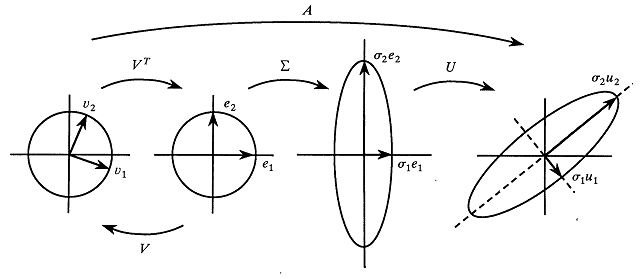
\includegraphics[scale=0.7]{img/svd1.png}
\end{remark}

\begin{theorem}[Proof of SVD]
	For $A\in\mathbb{R}^{m*n}$, consider symmetric matrix $A^\top A$ that has eigenvalues $\lambda_1 \cdots \lambda_r > 0$ with corresponding eigenvectors $v_1 \cdots v_r$ and $\lambda_{r+1} \cdots \lambda_n = 0$. Then we know that
	\[
	A^\top A\v{v}_i = \lambda_i\v{v}_i
	\]
	Let
	\[
	V = \begin{bmatrix}
	| & & | \\
	\v{v}_1 & \cdots & \v{v}_n\\
	| & & |
	\end{bmatrix}
	\] 
	Define $\sigma_i = \sqrt{\lambda_i}$, let 
	\[
A\v{v}_i = \sigma_i\v{u}_i \;\; i\le r
	\]
	for some vector $\v{u}_i$. \\ 

	\textbf{Claim.} $\v{u}_i$ are orthonormal.
	\begin{proof}
	\begin{align*}
		\v{u}_i^\top\v{u}_j &= \frac{(A\v{v}_i)^\top}{\sigma_i}\frac{(A\v{v}_j)}{\sigma_j} \\
		&= \frac{1}{\sigma_i \sigma_j}\v{v}_i^\top A^\top A \v{v}_j && A^\top A\v{v}_j = \lambda_j\v{v}_j\\
		&= \frac{1}{\sigma_i \sigma_j}\v{v}_i^\top \lambda_j\v{v}_j \\
		&= \frac{\lambda_j}{\sigma_i \sigma_j}\v{v}_i^\top \v{v}_j && \v{v}_i \v{v}_j \text{ orthonormal}\\
		&= \left\{\begin{array}{lr}
			0 & i\neq j \\
			1 & i =j
		\end{array}
	\end{align*}
	Therefore $\v{u}_i$ are orthonormal.
	\end{proof}
	Recall that A has rank r, we let
	\[
V_r = V = \begin{bmatrix}
	| & & | \\
	\v{v}_1 & \cdots & \v{v}_r\\
	| & & |
	\end{bmatrix}
	\]
	Hence
	\begin{align*}
		AV_r &= 
	\begin{bmatrix}
	| & & | \\
	\v{u}_1 & \cdots & \v{u}_r\\
	| & & |
	\end{bmatrix}\begin{bmatrix}
	\sigma_1 & & \\
	 & \ddots & \\
	 & & \sigma_r
	\end{bmatrix} = U_r\Sigma_r\\
	A&= U \Sigma V^\top
	\end{align*}
	Since V orthonormal and $V^{-1}=V^\top$
\end{theorem}

% subsection singular_value_decomposition (end)

 \vfill
\section{Vector Calculus} % (fold)
\label{sec:vector_calculus}

\begin{theorem}[Taylor's Theorem for Vectors]
	For $f(\v{x}):=\mathbb{R}^n\rightarrow\mathbb{R}$, the derivative of f is
	\[
f(\v{x}_0+\Delta\v{x}) = f(\v{x}_0)+\nabla f|^\top_{\v{x}=\v{x}_0}\Delta\v{x} + \frac{1}{2!}(\Delta\v{x})^\top\nabla^2f|_{\v{x}=\v{x}_0}\Delta\v{x}
	\]
	Where
	\begin{align*}
		\text{Gradient} &= \nabla f|^\top_{\v{x}=\v{x}_0}\\
		\text{Hessian} &= \nabla^2f|_{\v{x}=\v{x}_0}
	\end{align*}
	And
	\[
	f(\v{x}_0)+\nabla f|^\top_{\v{x}=\v{x}_0}\Delta\v{x}
	\]
	is the first-order approximation (a hyperplane). 
\end{theorem}

\begin{definition}[Gradient]
	The gradiant $\nabla f(\v{x})$ captures change according to all components of $\v{x}$. It is defined as
	\[
\nabla f(\v{x}) = \begin{bmatrix}
	\pd{f}{x_1} & \pd{f}{x_2} & \cdots & \pd{f}{x_n}
\end{bmatrix}
	\]
	The gradient always has the same dimension as the input vector.
\end{definition}

\begin{definition}[Hessian]
	The hessian is a matrix that captures the change according to all gradients. It is defined as
	\[
\nabla^2 f(\v{x})_{ij} = \frac{\partial f}{\partial x_i\partial x_j}
	\]
	Hessian is \textbf{often} symmetric.
\end{definition}

\begin{example}
	Let
	\[
f(\v{x}) = \|x\|_2^2, \;\; f:=\mathbb{R}^2\rightarrow\mathbb{R}
	\]
	Then the gradient of this function f is
	\[
\nabla f(\v{x}) = \begin{bmatrix}
	2x_1\\2x_2
\end{bmatrix} = 2\v{x}
	\]
	And the hessian is
	\[
\nabla^2 f(\v{x}) = \begin{bmatrix}
	2 & 0 \\ 0 & 2
\end{bmatrix}
	\]
	According to taylor theorem,
	\begin{align*}
		f(\v{x}+\Delta\v{x}) &= (x_1^2+x_2^2)+\begin{bmatrix}
	2x_1 &2x_2
\end{bmatrix}
\begin{bmatrix}
	\Delta x_1\\\Delta x_2
\end{bmatrix} + \frac{1}{2}\begin{bmatrix}
	\Delta x_1&\Delta x_2
\end{bmatrix}\begin{bmatrix}
	2 & 0 \\ 0 & 2
\end{bmatrix}\begin{bmatrix}
	\Delta x_1\\\Delta x_2
\end{bmatrix}\\
&= x_1^2+x_2^2+2x_1 \Delta x_1+2x_2 \Delta x_2 +\Delta x_1^2+ \Delta x_2^2\\
&= (x_1+\Delta x_1)^2 + (x_2+\Delta x_2)^2
	\end{align*}
\end{example}

\begin{example}
	Let
	\[
f(\v{x}) = \v{x}^\top\v{a} = \sum_{i=1}^nx_ia_i
	\]
	Then the gradient of this function f is
	\[
\nabla f(\v{x}) = \begin{bmatrix}
	a_1\\a_2\\\vdots\\a_n
\end{bmatrix} = \v{a}
	\]
	And the hessian is
	\[
\nabla^2 f(\v{x}) = 0
	\]
\end{example}

\begin{example}
	Let
	\[
f(\v{x}) = \v{x}^\top A\v{x}
	\]
	We can see that
	\begin{align*}
		f(\v{x}) &= \v{x}^\top A\v{x}\\
		&= \begin{bmatrix}
			x_1&\cdots&x_n
		\end{bmatrix}\begin{bmatrix}
			a_{11}&\cdots&a_{1n}\\
			\vdots&\ddots&\vdots\\
			a_{m1}&\cdots&a_{mn}
		\end{bmatrix}\begin{bmatrix}
			x_1\\\vdots\\x_n
		\end{bmatrix}\\
		&= \sum_i\sum_j x_ia_{ij}x_j
	\end{align*}
	Since all terms that contain $x_i$ is
	\[
\sum_{j\neq i}x_ia_{ij}x_j+\sum_{j\neq i}x_ja_{ji}x_i+x_i^2a_ii
	\]
	We know that
	\[
\frac{\partial f}{\partial x_i} = \sum_j(a_{ij}+a{ji})x_j
	\]
	Therefore the gradient of this function f is
	\[
\nabla f(\v{x}) = (A+A^\top)\begin{bmatrix}
	x_1\\\vdots\\x_n
\end{bmatrix} = (A+A^\top)\v{x}
	\]
	The hessian is 
	\[
\nabla^2 f(\v{x}) = A+A^\top
	\]
\end{example}

\begin{theorem}[The Main Theorem]
	Let $f:\mathbb{R}^n\rightarrow\mathbb{R}$ and f is differentiable everywhere. Consider the optimization problem subject to
	\[
\argmin_{\v{x},\;\v{x}\in \Omega} f(\v{x})
	\]
Where $\Omega$ is an open set in $\mathbb{R}^n$

Then if $\v{x}^*$ is an optimal solution, then
\[
\frac{df}{dx}(x^*) = 0
\]
Note that the converse is not necessarily true.
\end{theorem}

% section vector_calculus (end) \vfill
\section{Regression} % (fold)
\label{sec:regression}

\subsection{Sensitivity} % (fold)
\label{sub:sensitivity}

\begin{definition}[problem statement]
	Consider optimization problem
	\[
A\v{x} = \v{y}
	\]
	Under the special case that $A\in\mathbb{R}^{n*n}$ and is invertible. Now we apply a change to y such that $\v{y} \rightarrow \v{y}+\delta\v{y}$. Because of this, $\v{x} \rightarrow \v{x}+\delta\v{x}$. How big is $\delta\v{x}$?
\end{definition}

\begin{theorem}[condition number]
	The value we are interested in is $\frac{\| \delta \v{x}\|_2}{\|\v{x}\|_2}$. To investigate this value, we transform the equation such that
	\begin{align*}
	A(\v{x}+\delta\v{x}) &= \v{y}+\delta\v{y}\\
		A \delta\v{x} &= \delta\v{y}\\
		\delta\v{x}&=A^{-1}\delta\v{y}\\
		\|\delta\v{x}\|_2 &= \|A^{-1}\delta\v{y}\|_2
	\end{align*}
	Recall that
	\[
\|A\|_2 = \max_{\|y\|_2=1}\|A\v{y}\|_2 = \max_{y}\frac{\|A\v{y}\|_2}{\|y\|_2} = \sigma_{max}
	\]
	Therefore by the definition of the spectral norm,
	\[
\|\delta\v{x}\|_2 = \|A^{-1}\delta\v{y}\|_2 \le \|A^{-1}\|_2\|\delta\v{y}\|_2
	\]
	This gives us an upperbound of the solution. To find the lowerbound,
	\begin{align*}
		A\v{x}&=\v{y}\\
		\|\v{y}\|_2 &= \|A\v{x}\|_2 \le \|A\|_2\|\v{x}\|_2\\
		\|\v{x}\|_2 &\ge \frac{\|\v{y}\|_2}{\|A\|_2}
	\end{align*}
	Combining these two inequalities gives
	\begin{align*}
		\frac{\| \delta\v{x}\|_2}{\|\v{x}\|_2} &\le \frac{\|A^{-1}\|_2\| \delta\v{y}\|_2}{\|\v{y}\|_2/\|A\|_2}\\ 
		&\le \|A\|_2\|A^{-1}\|_2 \frac{\| \delta\v{y}\|_2}{\|\v{y}\|_2}\\
		&\le \left(\frac{\sigma_{max}}{\sigma_{min}}\right)\frac{\| \delta\v{y}\|_2}{\|\v{y}\|_2}
	\end{align*}
	The term $\frac{\sigma_{max}}{\sigma_{min}}$ is called the condition number of a matrix. If the condition number is large, a small change in y would cause a large change in x.
\end{theorem}

% subsection sensitivity (end)

\subsection{Shift property of eigenvalues} % (fold)
\label{sub:shift_property_of_eigenvalues}

\begin{theorem}[Shift property of eigenvalues]
	Consider matrix A. We add a diagonal matrix to A and change it to $A+\lambda I$. Then for $\lambda_1$ and $\v{v}_1$ be the first eigenpair of A,
	\[
(A+\lambda I)\v{v}_1 = A\v{v}_1+\lambda\v{v} = \lambda_1\v{v}_1+\lambda\v{v}_1=(\lambda_1+\lambda)\v{v}
	\]
	The eigenvalue of the new matrix $A+\lambda I$ is shifted by $\lambda$, but its eigenvector remain unchanged.
\end{theorem}

% subsection shift_property_of_eigenvalues (end)

\subsection{Ridge Regression} % (fold)
\label{sub:ridge_regression}

\begin{theorem}[Ridge regression]
	Consider the optimization problem
	\[
\min_{\v{x}}\|A\v{x}-\v{b}\|^2+\lambda^2\|\v{x}\|_2^2
	\]
	Where $\lambda^2\|\v{x}\|_2^2$ is called the \textbf{regularizer}. We have
	\begin{align*}
		f(\v{x}) &= (A\v{x}-\v{b})^\top(A\v{x}-\v{b})+\lambda^2\v{x}^\top\v{x}\\
		&= \v{x}^\top A^\top A\v{x}-\v{x}^\top A^\top \v{b}-\v{b}^\top A\v{x}+\lambda^2\v{x}^\top\v{x}+\v{b}^\top\v{b}
	\end{align*}
	The gradient of f is 
	\[
\nabla f(\v{x}) = 2A^\top A\v{x}-2(\v{b}^\top A)^\top +2 \lambda^2\v{x}
	\]
	Setting the gradient to zero gives us
	\begin{align*}
		(A^\top A+\lambda^2I)\v{x}^* &= A^\top\v{b}\\
\v{x}^* &= (A^\top A+\lambda^2 I)^{-1}A^\top\v{b}
	\end{align*} 

	Ridge regression has two interpretations.
	\begin{itemize}
		\item We want to shift the eigenvalues of A to limit the condition number so it is not too large.
		\item Without the regularizer, the predicted coefficient of the polynomial tend to be really large ($10^6$-level large). The regularizer integrated the size of x into the minimizing terms and controls the size of the predicted value so that it is not insanely large.
	\end{itemize}

	Note: the solution to the ridge regression is \textbf{not} the same as the solution to OLS. In general, these two solutions are distinct.
\end{theorem}

% subsection ridge_regression (end)

\subsection{Tikhonov regularization} % (fold)
\label{sub:tikhonov_regularization}

\begin{definition}[Tikhonov regularization]
	Consider data $A\v{x} = \v{b}$. We decide to add weights $W_1$ to the data points such that the weights represents the "importance" or "confidence." We then add some new data $W_2$ to A and a corresponding $\v{x}_0$ to $\v{b}$. With the additional information, the original data becomes:
	\[
W_1\begin{bmatrix}
	A \\ W_2
\end{bmatrix}\v{x} = \begin{bmatrix}
	\v{b} \\ \v{x}_0
\end{bmatrix}
	\]
	where $W_1$ and $W_2$ are matrices. The optimization problem becomes:
	\[
\min_{\v{x}}\|W_1(A\v{x}-\v{b})\|_2^2+\|W_2(\v{x}-\v{x}_0)\|_2^2
	\]
	Such problem is called Tikhonov regression.
\end{definition}

% subsection tikhonov_regularization (end)

\subsection{Probablistic perspective} % (fold)
\label{sub:probablistic_perspective}

\begin{definition}[Problem statement]
	Consider model
	\[
y_i = g(x_i)+z_i
	\]
	Where $z_i$ is noise. We have some information about the noise such that 
	\[
z_i \sim N(0,\sigma_i^2) \rightarrow f(z_i) = \frac{e^{-z_i^2/2\sigma_i^2}}{\sqrt{2\pi}\sigma_i}
	\]
	This model is our data points. \textbf{Assume} the model is linear, i.e. $g(\v{x}_i) = \v{x}_i^\top\v{w}$. In this context, we can call $\v{w}$ as our "model". We can rewrite the original equation to
	\[
\begin{bmatrix}
	y_1\\\vdots\\y_n
\end{bmatrix} = \begin{bmatrix}
	\cdots&\v{x}_1^\top&\cdots\\
	&\vdots&\\
	\cdots&\v{x}_n^\top&\cdots
\end{bmatrix}\v{w}+\begin{bmatrix}
	z_1\\\vdots\\z_n
\end{bmatrix}
	\]
	such that $\v{y}\approx X\v{w}$. We could solve this problem by OLS, but OLS does not count into consideration the information we know about the noise and thus gives suboptimal solution. Is there a better way to choose $\v{w}$?
\end{definition}

\begin{theorem}[Maximum Likelihood estimation]
	Goal: find $\v{w}$ that makes observed data most likely, i.e.
	\[
\argmax_{\v{w}_0} f(Y_1 = y_1,\cdots,Y_n=y_n|\v{w} = \v{w}_0)
	\]
	Assume $z_i$ i.i.d. Then we can rewrite the original problem into
	\[
\argmax_{\v{w}_0}\prod_{i=1}^nf(Y_i=y_i|\v{w} = \v{w}_0)
	\]
	Note that
	\begin{align*}
		f(Y_i=y_i|\v{w}=\v{w}_0) &= f(\v{x}_i^\top\v{w}_0+z_i=y_i|\v{w}=\v{w}_0\\
		&= f(z_i=y_i-\v{x}_i^\top\v{w}_0|\v{w}=\v{w}_0)\\
		&= \frac{e^{\frac{-(y_i-\v{x}_i^\top\v{w}_0)^2}{2\sigma_i^2}}}{\sqrt{2\pi}\sigma_i}
	\end{align*}
	Therefore
	\begin{align*}
	\argmax_{\v{w}_0}\prod_{i=1}^nf(Y_i=y_i|\v{w} = \v{w}_0) &= \argmax_{\v{w}_0}\prod_{i=1}^n\frac{e^{\frac{-(y_i-\v{x}_i^\top\v{w}_0)^2}{2\sigma_i^2}}}{\sqrt{2\pi}\sigma_i}\\
		&= \argmax_{\v{w}_0} \frac{1}{(\sqrt{2\pi})^n\prod_{i=1}^n\sigma_i} \prod_{i=1}^ne^{\frac{-(y_i-\v{x}_i^\top\v{w}_0)^2}{2\sigma_i^2}}\\
		&= \argmax_{\v{w}_0} \frac{1}{(\sqrt{2\pi})^n\prod_{i=1}^n\sigma_i} \exp\left\{-\sum_{i=1}^n\frac{-(y_i-\v{x}_i^\top\v{w}_0)^2}{2\sigma_i^2}\right\}\\
		&= \argmax_{\v{w}_0} -\sum_{i=1}^n\frac{-(y_i-\v{x}_i^\top\v{w}_0)^2}{2\sigma_i^2}\\
		&= \argmin_{\v{w}_0} \sum_{i=1}^n\frac{-(y_i-\v{x}_i^\top\v{w}_0)^2}{2\sigma_i^2}\\
		&= \argmin_{\v{w}_0} \|S(X\v{w}_0-\v{y})\|^2_2
	\end{align*}
	Where
	\[
S = \begin{bmatrix}
			\sqrt{\frac{1}{2 \sigma_1^2}} &&\\
			&\ddots&\\
			&&\sqrt{\frac{1}{2 \sigma_n^2}}
	\end{bmatrix}
	\]
\end{theorem}

\begin{theorem}[Maximum a posteriori estimation (MAP)]
	Based on the problem stated in MLE, what if we have a prior on $\v{w}$? Again, we have
	\[
y_i = g(x_i)+z_i
	\]
	\[
z_i \sim N(0,\sigma_i^2) \rightarrow f(z_i) = \frac{e^{-z_i^2/2\sigma_i^2}}{\sqrt{2\pi}\sigma_i}
	\]
	In addition,
	\[
w_i \sim N(\mu_i,\rho_i^2)
	\]
	i.e.
	\[
\v{w} \sim N(\v{\mu}, \Sigma_{\v{w}}) \;\; s.t.\;\; \Sigma_{\v{w}} = \begin{bmatrix}
	\rho_1^2 &&\\
	&\ddots&\\
	&&\rho_n^2
\end{bmatrix}
	\]
	Goal: find the most likely $\v{w}$ given data $y_1, \cdots, y_n$, i.e.
	\[
\argmax_{\v{w}} f(\v{w}|\v{Y} = \v{y})
	\]
	By the Bayes theorem,
	\[
	f(\v{w}|\v{Y} = \v{y}) = \frac{f(\v{Y}=\v{y}|\v{w})f{\v{w}}}{f{\v{Y}}}
	\]
	Hence
	\begin{align*}
		\argmax_{\v{w}} f(\v{w}|\v{Y} = \v{y}) &= \argmax_{\v{w}} f(\v{Y}=\v{y}|\v{w})f(\v{w})\\
		&= \argmax_{\v{w}} \left(\prod_{i=1}^nf(Y=y_i|\v{w})\right)f(\v{w})
	\end{align*}
	Borrowing the calculation we did in MLE,
	\begin{align*}
		\argmax_{\v{w}} f(\v{w}|\v{Y} = \v{y}) &= \argmax_{\v{w}} \prod_{i=1}^n
		\frac{\exp\left\{\frac{-(y_i-\v{x}_i^\top\v{w}_0)^2}{2\sigma_i^2}\right\}}{\sqrt{2\pi}\sigma_i}\frac{\exp\left\{-(\v{w}-\v{\mu})^\top\Sigma_W^{-1}(\v{w}-\v{\mu})\right\}}{(\sqrt{2\pi})^n(\prod\rho_i)}\\
		&= \argmax_{\v{w}} \exp\left\{\sum_{i=1}^n \frac{-(y_i-\v{x}_i^\top\v{w}_0)^2}{2\sigma_i^2} -(\v{w}-\v{\mu})^\top\Sigma_W^{-1}(\v{w}-\v{\mu}) \right\}\\
		&= \argmax_{\v{w}} \sum_{i=1}^n \frac{-(y_i-\v{x}_i^\top\v{w}_0)^2}{2\sigma_i^2} -(\v{w}-\v{\mu})^\top\Sigma_W^{-1}(\v{w}-\v{\mu})\\
		&= \argmin_{\v{w}} \sum_{i=1}^n \frac{(y_i-\v{x}_i^\top\v{w}_0)^2}{2\sigma_i^2} +(\v{w}-\v{\mu})^\top\Sigma_W^{-1}(\v{w}-\v{\mu})\\
		&= \argmin_{\v{w}} \|S(X\v{w}_0-\v{y})\|^2_2 + \|\sqrt{\Sigma_W^{-1}}(\v{w}-\v{\mu})\|_2^2
	\end{align*}
	For example, if some $\rho$'s are large (note that $\rho$'s are the variances of the w's), you do not need to care too much about keeping w and $\mu$ close in their values. But if $\rho$'s are small, than differences in values of w and $\mu$ are going to have a large impact (Therefore you should put a high weight on keeping w and $\mu$ similar).

\end{theorem}

% subsection probablistic_perspective (end)

% section regression (end) \vfill
\section{Convexity} % (fold)
\label{sec:convexity}

\subsection{Convex Sets} % (fold)
\label{sub:convex_sets}



% subsection convex_sets (end)

% section convexity (end) \vfill
\section{Gradient Descent} % (fold)
\label{sec:gradient_descent}

\begin{definition}[Gradient Descent]
	Gradient Descent is an approach to unconstrained optimization problems. The basic idea is to nudge the function in the right direction by a little bit in every step, and after a lot of steps the function will arrive at a local minimum. Formally, for a step size s and a direction $\v{v}$,
	\[
f(\v{x}+s\v{v}) \approx f(\v{x})+s<\nabla f(\v{x}), \v{v}>
	\]
	Recall Cauchy-Schwartz, the magnitude of $<\nabla f(\v{x}), \v{v}>$ is maximized if $\v{v}$ is aligned with $\nabla f(\v{x})$. We want to minimize the inner product while maximize its magnitude so the function steps towards the minimum at the fastest rate, hence we choose
	\[
\v{v} = -\nabla f(\v{x})
	\]
	The formal algorithm for gradiant descent is defined as follows. Let $\v{x}$ be the parameter of function f. At step k,
	\[
\v{x}_{k+1} = \v{x}_k -\eta\nabla f(\v{x}_k)
	\]
	Where $\v{x}_0$ is the initial point and $\eta$ is the stepsize.
\end{definition}

\begin{example}[GD on LS]
	Let $f(\v{x}) = \|A\v{x}-\v{b}\|_2^2$. It has a direct solution of $\v{x}^* = (A^\top A)^{-1}A^\top\v{b}$. If A is a n*n matrix, the runtime of computing the direct solution is at least $O(n^3)$ (taking a matrix inverse is approx. $O(n^3)$). It is computationally cheaper to use gradient descent. Thus,
	\[
\nabla f(\v{x}) = 2A^\top(A\v{x}-\v{b})
	\]
\begin{align*}
	\v{x}_{k+1} &= \v{x}_k -\eta\nabla f(\v{x}_k)\\
	&= \v{x}_k - \eta 2A^\top(A\v{x}-\v{b})\\
	\v{x}_{k+1} &= (I-2\eta A^\top A)\v{x}_k + 2\eta A^\top\v{b}
\end{align*}
	Next we need to prove that this algorithm will converge. The following is one of the ways to prove convergence. The difference between optimal value and the k-step value is
	\begin{align*}
		\v{x}_{k+1} - (A^\top A)^{-1}A^\top\v{b} &= (I-2\eta A^\top A)\v{x}_k + 2\eta A^\top\v{b} - (A^\top A)^{-1}A^\top\v{b}\\
		&= (I-2\eta A^\top A)\v{x}_k + 2\eta(A^\top A)(A^\top A)^{-1}A^\top\v{b}-(A^\top A)^{-1}A^\top\v{b}\\
		&= (I-2\eta A^\top A)\v{x}_k + (2\eta A^\top A-I)(A^\top A)^{-1}A^\top\v{b}\\
		&= (I-2\eta A^\top A)(\v{x}_k - (A^\top A)^{-1}A^\top\v{b})
	\end{align*}
	Hence if the absolute values of the eigenvalues of $I-2\eta A^\top A$ are strictly less than 1, GD converges for LS.
\end{example}

% section gradient_descent (end) \vfill
\section{Duality} % (fold)
\label{sec:duality}

\subsection{Weak Duality} % (fold)
\label{sub:weak_duality}

\begin{remark}
	Gradient Descent works for unconstrained optimization problem on convex functions. It has challenges that the function should be differentiable and convex, and at the same time GD is computationally expensive. 

	Duality is a technique that transforms every problem to a convex form (the dual form). It does not necessarily give us the solution to the original problem, but it will always give a bound.
\end{remark}

\begin{theorem}[Lagrangian]
	Optimization problem
	\[
p^* = \min f_0(\v{x})
	\]
	Under the constrains
	\begin{align*}
		f_i(\v{x})&\le0,\;\;\;\forall i\;\;1\le i\le m\\
		h_i(\v{x})&=0,\;\;\;\forall i\;\;1\le i\le p
	\end{align*}
	The problem defined above is called a \textbf{primal problem}. Define \textbf{Lagrangian}:
	\[
L(\v{x},\v{\lambda},\v{\nu}) = f_0(\v{x})+\sum_{i=1}^m \lambda_if_i(\v{x})+\sum_{i=1}^p\nu_ih_i(\v{x}) \;\;\; \forall \lambda_i \ge 0
	\]
	Note that it is an \textbf{affine} function of $\lambda$ and $\nu$, which means that it is \textbf{both convex and concave}. Now, define new problem
	\[
\min_{\lambda \ge 0} L(\v{x},\v{\lambda},\v{\nu}) := g(\v{\lambda},\v{\nu})
	\]
	Over all $\v{x}$. Examine g. Properties of g include
	\begin{enumerate}
		\item g is a function of only $\v{\lambda},\v{\nu}$.
		\item L is an affine function of $\v{\lambda},\v{\nu}$.
		\item By 1 and 2, g is a concave function of $\v{\lambda},\v{\nu}$.
		\item It turns out, \textbf{g($\v{\lambda},\v{\nu}$) is a lower bound on the primal optimal $p^*$}.
	\end{enumerate}
\end{theorem}
Proof of property No. 4: TODO

\begin{example}[Duality on LS]
	Let $A\in\mathbb{R}^{m*n}$, $m<n$. Problem
	\[
\min \v{x}^\top\v{x} = \v{p}^*
	\]
	Under the constrain
	\[
A\v{x} = \v{b}
	\]
	Since there is no inequality constains, the lagrangian of this problem does not have $\lambda$.
	\[
L(\v{x},\v{\nu}) = \v{x}^\top\v{x} + \nu^\top(A\v{x}-\v{b})
	\]
	\[
g(\v{\nu}) = \min_{\v{x}}L(\v{x},\v{\nu})
	\]
	To solve for g, we do
	\[
\nabla_{\v{x}} L(\v{x},\v{\nu}) = 2\v{x}+A^\top\v{\nu}
	\]
	Set gradient to zero,
	\[
\v{x} = -\frac{1}{2}A^\top\v{\nu}
	\]
	Is the point where L is minimized. g at this point is 
	\begin{align*}
		g(\v{\nu}) &= L(-\frac{1}{2}A^\top\v{\nu}, \v{\nu}) = (-\frac{1}{2}A^\top\v{\nu})^\top(-\frac{1}{2}A^\top\v{\nu})+\v{\nu}^\top(-\frac{1}{2}AA^\top\v{\nu}-\v{b})\\
		&=\frac{1}{4}\v{\nu}^\top A A^\top\v{\nu} +\v{\nu}^\top(-AA^\top\v{\nu}-\v{b})\\
		&= -\frac{1}{4}\v{\nu}^\top A A^\top\v{\nu} - \v{\nu}^\top\v{b}
	\end{align*}
	Which is the lower bound of $p^*$. What is the max lower bound? In another word, we want to find
	\[
\max_{\v{\nu}}g(\v{\nu})
	\]
	Since g concave, we take its gradient and set to zero:
	\begin{align*}
		\nabla_{\v{\nu}} g(\v{\nu}) &= -\frac{1}{4}2AA^\top\v{\nu}-\v{b} = 0\\
		\v{\nu}^* &= -2(AA^\top)^{-1}\v{b}
	\end{align*}
	Thus
	\[
\v{x}^* = -\frac{1}{2}A^\top(-2(AA^\top)^{-1}\v{b}) = A^\top(AA^\top)^{-1}\v{b}
	\]
\end{example}

\begin{definition}[Dual]
	Continuing the definition of lagrangian, we want to find the tightest lower bound of $p^*$, formally
	\[
\max_{\v{\lambda}\ge0}g(\v{\lambda},\v{\nu}) = d^*
	\]
	Over $\v{\nu}$, this problem is the \textbf{DUAL Problem}. It is a maximization problem of a concave function under linear constrains, thus a \textbf{convex program}.
\end{definition}

\begin{remark}
	Properties of the Dual problem:
	\begin{enumerate}
		\item \# of variables = \# of constraints of the primal.
		\item \textbf{Always convex problem even if primal is not! :)}
	\end{enumerate}
	By 1, if the data is large but the constaints are few, the Dual problem is an easier problem to solve.
\end{remark}

\begin{definition}[Weak Duality]
	Continuing from the definition of lagrangian and duality, if
	\[
d^*\le p^*
	\]
	Then it is \textbf{WEAK DUALITY}.
\end{definition}

% subsection weak_duality (end)

\subsection{Strong Duality} % (fold)
\label{sub:strong_duality}

\begin{definition}[Strong Duality]
	If
	\[
d^*= p^*
	\]
	Like we seen in the Duality on LS example, then it is \textbf{STRONG DUALITY}.
\end{definition}

\begin{remark}
	Strong Duality $\implies$ Weak Duality. \textbf{In general, weak duality always holds}, while strong duality only holds under certain circumstances.
\end{remark}

\begin{definition}[duality gap]
	\[
p^*-d^*
	\]
	is called the duality gap. Duality gap = 0 iff strong duality.
\end{definition}

\begin{theorem}[Minmax Inequality]
	Sets X, Y. F is any function. Then,
	\[
\min_{x\in X} \max_{y\in Y} F(x, y) \ge \max_{y\in Y} \min_{x\in X} F(x, y)
	\]
\end{theorem}
Proof of Minmax Inequality:
\begin{proof}
	Fix $x_0\in X$, $y_0\in Y$. Define
	\[
h(y_0) := \min_{x\in X}F(x, y_0)
	\]
	and
	\[
g(x_0) := \max_{y\in Y}F(x_0, y)
	\]
	See that
	\[
h(y_0) = \min_{x\in X}F(x, y_0) \le F(x_0, y_0) \le \max_{y\in Y}F(x_0, y) = g(x_0)
	\]
	Thus
	\begin{align*}
		h(y_0) &\le g(x_0) \\
		\max_{y\in Y} h(y_0) &\le \min_{x\in X}g(x_0)\\
		\max_{y\in Y} \min_{x\in X} F(x, y) &\le \min_{x\in X} \max_{y\in Y} F(x, y)
	\end{align*}
\end{proof}

\begin{remark}[Implication of Minmax Inequality on Duality]
	By definition,
\begin{align*}
	d^* &= \max_{\v{\lambda}\ge0}g(\v{\lambda},\v{\nu})\\
	&= \max_{\v{\lambda}\ge0} \min_{\v{x}} L(\v{x},\v{\lambda},\v{\nu})
\end{align*}
How can we connect this to the primal? Consider
\begin{align*}
	&\max_{\v{\lambda}\ge0,\;\v{\nu}} \left(f_0(\v{x})+\sum_{i=1}^m \lambda_if_i(\v{x})+\sum_{i=1}^p\nu_ih_i(\v{x})\right)\\
	=&\begin{cases}
		f_0(\v{x}) & \text{if }\v{x} \text{ is feasible}\\
		\infty& \text{if }\v{x} \text{ is infeasible}
	\end{cases}
\end{align*}
Therefore we can write
\[
p^* = \min_{\v{x}}\max{\v{\lambda}\ge0,\;\v{\nu}} L(\v{x}, \v{\lambda}, \v{\nu})
\]
By the minmax inequality,
\[
p^* \ge d^*
\]
\end{remark}

\begin{theorem}[Slater's Condition]
	For a convex problem, strong duality holds if 
	\[
\exists \v{x}_0 \text{ such that } f_i(\v{x}_0) < 0 \;\;\forall i
	\]
	In another word, the point $\v{x}_0$ is strictly feasible. Or,
	\[
\v{x}_0 \in \text{ RelativeInterior}(\mathbf{D})
	\]
	For the purpose of this class we can think of RelativeInterior as the Interior.
\end{theorem}

\begin{theorem}[Refined Slater's Condition]
	Convex problem, $\li{f}{k}$ that are affine,
	\[
\exists \v{x}_0 \text{ such that } f_i(\v{x}_0) \le 0 \;\;\forall i = 1, 2, \cdots, k \text{ AND } f_i(\v{x}_0) < 0\;\;\forall i = k+1,\cdots, m
	\]
	Assume that first k constraints are affine, and the rest are whatever non-linear things that you want them to be. You are allowed to have equality for the affine things, as long as the non-affine things all satisfy the above strict inequality. So you don't have to find a point that satisfies strict inequalities on the affine things too. Sometimes it is easier to find such point.
\end{theorem}

\begin{remark}
	As long as the problem is feasible, strong duality will always hold for linear program.
\end{remark}

% subsection strong_duality (end)
\newpage
\subsection{Partitioning Problem} % (fold)
\label{sub:partitioning_problem}

\begin{definition}[partitioning problem]
	\[
\min_{\v{x}_i,\;\v{x}_i^2 = 1} \v{x}^\top W\v{x},\;\;W\in \mathbb{S}^n
	\]
\end{definition}

\begin{remark}
	Partitioning problem is not a convex problem. This is because that $\v{x}_i$ can only be either +1 or -1, thus the domain is descrete.
\end{remark}

The lagrangian for the partitioning problem is 
\begin{align*}
	L(\v{x},\v{\nu}) &= \v{x}^\top W\v{x} + \sum_{i=1}^n\v{\nu}_i(\v{x}_i^2-1)\\
	&= \v{x}^\top W\v{x} + \v{x}^\top diag(\v{\nu})\v{x} - \sum_{i=1}^n\v{\nu}_i\\
	&= \v{x}^\top(W+diag(\v{\nu}))\v{x} - \sum_{i=1}^n\v{\nu}_i
\end{align*}
If $(W+diag(\v{\nu}))$ is PSD, the problem is convex. If it is NSD, the problem is concave. The g for the partitioning problem is
\begin{align*}
	g(\v{\nu}) &= \min_{\v{x}}L(\v{x},\v{\nu})\\
	&= \begin{cases}
		-\sum_{i=1}^n\v{\nu}_i  &\text{if $(W+diag(\v{\nu}))$ PSD}\\
		-\infty &\text{otherwise}
	\end{cases}
\end{align*}
We see that this problem is trivial if $(W+diag(\v{\nu}))$ is not PSD. We can rewrite this problem as its dual:
\[
\max \sum_{i=1}^n\v{\nu}_i,\;\;\text{subject to}\;\;(W+diag(\v{\nu}))\succeq 0
\]
This is a special kind of problem called \textbf{Semi-definite Program}. It is a convex problem that can be efficiently solved. Particularly, for this problem, we choose
\[
\v{\nu} = \lambda_{min}(W)
\]
and we have the lower bound
\[
p^* \ge n \lambda_{min}(W)
\]
This is an example of transforming a very hard-to-solve problem into a convex problem that we can efficiently solve.

% subsection partitioning_problem (end)
\newpage 
\subsection{LP and Duality} % (fold)
\label{sub:lp_and_duality}

\begin{example}
	Consider linear program
	\[
\min_{A\v{x}\le \v{b}} \v{c}^\top\v{x}
	\]
	The lagrangian is
	\begin{align*}
		L(\v{x},\v{\lambda}) &= \v{c}^\top\v{x}+\v{\lambda}^\top(A\v{x}\le \v{b})\\
		&= (A^\top\v{\lambda}+\v{c})^\top\v{x}-\v{b}^\top\v{\lambda}
	\end{align*}
	The g is 
	\begin{align*}
		g(\v{\lambda}) &= \min_{\v{x}}L(\v{x},\v{\lambda})\\
		&= \begin{cases}
			-\infty & \text{if } A^\top\v{\lambda}+\v{c}\neq 0\\
			-\v{b}^\top\v{\lambda} & \text{if } A^\top\v{\lambda}+\v{c}= 0
		\end{cases}
	\end{align*}
	The first case is trivial. In order to get a non-trivial bound, we want to calculate
	\[
d^* = \max_{\v{\lambda}\ge0,\;A^\top\v{\lambda}+\v{c}=0} -\v{b}^\top\v{\lambda}
	\]
	This is our dual problem.

\end{example}

\begin{example}[Winery]
	Consider the following business problem. You have 200 kilos of merlot and 300 kilos of shiras. You have two recipes:
	\begin{itemize}
		\item Blend 1: 4 kilos merlot + 1 kilo shiras, sell \$20
		\item Blend 2: 2 kilos merlot + 3 kilos shiras, sell \$15
	\end{itemize}
	You want to make $q_1$ of blend 1 and $q_2$ of blend 2. How to optimize our revenue? We set up problem for this
	\[
\max_{q_1,\; q_2 \ge 0} 20q_1 +15q_2
	\]
	Subject to
	\begin{align*}
		4q_1+2q_1&\le 200\\
		q_2+3q_2&\le 300
	\end{align*}
	Let's say we sell the leftover grapes. Let $\lambda_1$ be the rate to sell marlot and $\lambda_2$ be the rate to sell shiras. Then we write new optimization problem
	\begin{align*}
		&\max_{q_1,\; q_2 \ge 0} 20q_1 +15q_2 +\lambda_1(200-4q_1+2q_1) +\lambda_2(300-q_2+3q_2)\\
		=& \max_{q_1,\; q_2 \ge 0} (20-4 \lambda_1- \lambda_2)q_1+(15-2 \lambda_1-3 \lambda_2)q_2+200 \lambda_1+300 \lambda_2
	\end{align*}
	Note that the first line looks like a lagrangian. From the second line we can see that
	\begin{itemize}
		\item if $(20-4 \lambda_1- \lambda_2)$ negative, do not make blend 1. If it is positive, make as much blend 1 as you can.
		\item if $(15-2 \lambda_1-3 \lambda_2)$ negative, do not make blend 2. If it is positive, make as much blend 2 as you can.
	\end{itemize}
	The strategy seems clear. But what if we have
	\[
20-4 \lambda_1- \lambda_2 = 0 \text{ AND } 15-2 \lambda_1-3 \lambda_2 = 0
	\]? Then we do not care whether to sell the grapes or to make grapes into wine. These lambda's are called the \textbf{shadow prices} of grapes. What is our minimum revenue under these conditions? It is
	\[
\min_{\lambda_1, \; \lambda_2 \ge 0} 200 \lambda_1+300 \lambda_2
	\]
	Subject to
	\[
20-4 \lambda_1- \lambda_2 = 0 \text{ AND } 15-2 \lambda_1-3 \lambda_2 = 0
	\]
	If plug in the numbers, you can see that the original problem and the shadow price problem are primal and dual of each other. Note that for this particular problem, the feasible region of the dual problem is a point.
\end{example}

% subsection lp_and_duality (end)

\subsection{Duality Certificates} % (fold)
\label{sub:duality_certificates}

\begin{definition}[certificate]
	Let $(\lambda_1, \nu_1)$ be a dual feasible point, meaning that it satisfy the constaints of the dual. Let $x_1$ be the primal feasible point. Then we know that
	\[
p^* \ge g(\lambda_1, \nu_1)
	\]
	This implies that
	\[
f_0(x_1)-p^* \le f_0(x_1)-g(\lambda_1, \nu_1)
	\]
	This means that if $f_0(x_1)-g(\lambda_1, \nu_1)$ is small, $f_0(x_1)-p^*$ is also small. This could be used as the stopping condition for optimization programs. Another way of writing this is that
	\[
p^* \in [g(\lambda_1, \nu_1), f_0(x_1)]
	\]
	If the strong duality holds, we would also have
	\[
d^* \in [g(\lambda_1, \nu_1), f_0(x_1)]
	\]
	Note that if the strong duality does not hold, the above about $d^*$ might not be true due to possibly large duality gap.
\end{definition}

% subsection duality_certificates (end)

\subsection{Complementary Slackness} % (fold)
\label{sub:complementary_slackness}

\begin{theorem}[complementary slackness]
	Consider the following situation: the primal optimal $\v{x}^*$ and dual optimal $\v{\lambda}^*, \v{\nu}^*$. Assume strong duality holds, i.e. $p^*=d^*$. We have
	\[
p^* = f_0(\v{x}^*) = d^* = g(\v{\lambda}^*, \v{\nu}^*)  
	\]
	And
	\begin{align*}
		g(\v{\lambda}^*, \v{\nu}^*) &= \min_{\v{x}} \left(f_0(\v{x})+\sum_{i=1}^m \lambda_i^*f_i(\v{x})+\sum_{i=1}^p\nu_i^*h_i(\v{x})\right)\\
		&\le f_0(\v{x}^*) + \sum_{i=1}^m \lambda_i^*f_i(\v{x}^*)+\sum_{i=1}^p\nu_i^*h_i(\v{x}^*) \tag{1}
	\end{align*}
	Since we are considering primal problem with constraints including $f_i(\v{x})\le 0$ and the dual $d^* = \max_{\v{\lambda}\ge 0}g(\v{\lambda},\v{\nu})$, we know the term $\sum_{i=1}^m \lambda_i^*f_i(\v{x}^*)$ is at most zero. In addition, the constraints of the primal problem includes $h_i(\v{x})= 0$ and thus $\sum_{i=1}^p\nu_i^*h_i(\v{x}^*)$ is zero. Therefore we could write
	\begin{align*}
		g(\v{\lambda}^*, \v{\nu}^*) &\le f_0(\v{x}^*) +0 +0 = f_0(\v{x}^*) \tag{2}
	\end{align*}
	If the above holds, then both inequalities (1) and (2) must in fact be equalities!
\end{theorem}

Proof of Complementary Slackness: TODO

% subsection complementary_slackness (end)

\subsection{KKT Conditions} % (fold)
\label{sub:kkt_conditions}

\begin{remark}
	Karush-Kuhn-Tucker are the three people responsible for these conditions.
\end{remark}

\begin{theorem}[KKT Conditions]
	The following enumerated conditions are \textit{necessary}, but not necessarily \textit{sufficient}, conditions to the optimality of primal optimal $\v{x}^*$ and dual optimal $\v{\lambda}^*, \v{\nu}^*$. Assume strong duality holds, i.e. $p^*=d^*$. Convex OR non-convex problem. Both object function and the contraints differentiable. Then, the fact that primal optimal $\v{x}^*$ and dual optimal $\v{\lambda}^*, \v{\nu}^*$ implies
	\begin{enumerate}
		\item $f_i(\v{x}^*) \le 0\;\; \forall i=1,\cdots,m$
		\item $h_i(\v{x}^*) = 0\;\; \forall i=1,\cdots,p$
		\item $\lambda_i^* \ge 0 \;\; \forall i=1,\cdots,m$
		\item $\lambda_i^*f_i(\v{x}^*) = 0 \;\; \forall i=1,\cdots,m$ (Complementary Slackness)
		\item $\nabla f_0(\v{x}^*)+\sum \lambda_i^*\nabla f_i(\v{x}^*) +\sum\nu_i^*\nabla h_i(\v{x}^*) = 0$
	\end{enumerate}
	The fifth condition means that $\v{x}^*$ minimizes $L(\v{x},\v{\lambda}^*,\v{\nu}^*)$, which is implied by the Main Theorem.
\end{theorem}

\begin{theorem}[KKT Conditions Part II]
	Convex and differentiable problems. Strong duality not necessarily holds. Sufficient conditions. $\tilde{x}, \tilde{\lambda}, \tilde{\nu}$ are points. f's are convex and h's are affine. If the points satisfy:
	\begin{enumerate}
		\item $f_i(\tilde{x}) \le 0\;\; \forall i=1,\cdots,m $
		\item $h_i(\tilde{x}) = 0\;\; \forall i=1,\cdots,p$
		\item $\tilde{\lambda}_i \ge 0 \;\; \forall i=1,\cdots,m$
		\item $\tilde{\lambda}_if_i(\tilde{x}) = 0 \;\; \forall i=1,\cdots,m$
		\item $\nabla f_0(\tilde{x})+\sum \tilde{\lambda}_i\nabla f_i(\tilde{x}) +\sum\tilde{\nu}_i\nabla h_i(\tilde{x}) = 0$
	\end{enumerate}
	Then $\tilde{x}, \tilde{\lambda}, \tilde{\nu}$ are primal+dual optimal. Note that the strong duality is not needed for sufficiency only, but for it to be an iff statement you need strong duality: 
	\[
\text{optimality} \iff \text{the points satisfy KKT + problem convex + $h_i$ affine + slater conditions}
	\]
\end{theorem}
Proof of KKT Conditions: TODO

% subsection kkt_conditions (end)

% section duality (end) \vfill
\section{Linear Programs} % (fold)
\label{sec:linear_programs}

\begin{remark}
		\[
\v{a}^\top\v{x} = \v{b} \iff \v{a}^\top\v{x} \le \v{b} \;\;AND\;\; \v{a}^\top\v{x} \ge \v{b}
	\]
\end{remark}

\begin{theorem}
	All LP's can be translated into the following standard form:
	\[
\min_{A\v{x} = \v{b}\;\;\v{x}\ge 0} \v{c}^\top\v{x}
	\]
	1. How to \textbf{eliminate inequality}? For expression
	\[
\sum_{j=1}^na_{ij}x_j \le b
	\]
	We can rewrite it as
	\[
\sum_{i=1}^na_{ij}x_j+S_i=b_i, \;\; S_i \ge 0
	\]
	2. How to get $x_i\ge0$ for all $x_i$? If $x_i$ is unconstrained, we can always express it as the difference of two positive numbers: $x_i = x_i^+-x_i^-$. For example:
	\begin{align*}
		&\min2x_1+4x_2\\
		s.t.\;\;&x_1+x_2\ge3\\
		&3x_1+2x_2=14\\
		&x_1\ge0
	\end{align*}
	We can express the constraints by introducing a slack variable $x_3$\begin{align*}
		x_1+x_2-x_3&=3\;\;x_3\ge0\\
		x_2&=x_2^+-x_2^-\\
	\end{align*}
	By doing this we can rewrite the original problem as
	\begin{align*}
		&\min2x_1+3x_2^+-4x_2^-\\
		s.t.\;\;&x_1+x_2^+-x_2^--x_3 = 3\\
		&3x_1+2x_2^+-2x_2^- = 14\\
		&x_1\ge0\\
		&x_2^+\ge0\\
		&x_2^-\ge0\\
		&x_3\ge0
	\end{align*}
\end{theorem}

\begin{definition}[Polyhedron]
\[
Set \{\v{x}\in\mathbb{R}^n \;|\; A\v{x} \ge \v{b}\} \;A\in\mathbb{R}^{m*n}\;\;\v{b}\in\mathbb{R}^m
\]
Is called a polyhedron. Standarf form:
\[
Set\{\v{x}\in\mathbb{R}^l \;|\;c\v{x}=\v{d};\;\v{x}\ge0 \}
\]
Intuitively, P is the feasible region of a LP.
\end{definition}

\begin{definition}[Extreme points of a polyhedron]
	$x\in P$ is an extreme point (i.e. vertex of P) if we cannot find two vectors $\v{y},\v{z}\neq\v{x},\;\v{y},\v{z}\in P$ and $\lambda\in[0,1]$ such that $\v{x}=\lambda\v{y}+(1- \lambda)\v{z}$.

	\noindent That is, a point x is a vertex iff we cannot find two other point on this polyhedron such that these two points form a convex combination of x.
\end{definition}

\begin{theorem}
	P has an extreme point iff P does not contain a line.
\end{theorem}

\begin{theorem}
	Consider
	\[
\min_{A\v{x}\le\v{b}} \v{c}^\top\v{x}
	\]
	Assume 1. P has an extreme point, 2. optimal solution exists and is finite. Then there exists an optimal solution that is an extreme point of P. (Note that this is not saying all solutions are extreme points.)
\end{theorem}
Proof of theorem 7.6: TODO
% section linear_programs (end) \vfill
\section{Quadratic Programs} % (fold)
\label{sec:quadratic_programs}

\subsection{Solutions to QP} % (fold)
\label{sub:solutions_to_qp}

\begin{definition}
	\begin{align*}
	&\min \frac{1}{2}\v{x}^\top H\v{x} +\v{c}^\top\v{x}\\
	s.t.\;\;&A\v{x}\le\v{b}\\
	&C\v{x} = \v{d}
\end{align*}
Is a quadratic program. In general, QPs are not convex. However, if $H = H^\top$ and $H$ is PSD, then this is also convex.
\end{definition}

\begin{definition}[Moore-Penrose Pseudoinverse]
	Let H be n*n matrix, $H = U\Sigma V^\top$, H has rank r, then
	\[
H = U \begin{bmatrix}
	\Sigma_{r*r}&0\\0&0
\end{bmatrix}V^\top
	\]
	Then the Moore-Penrose Pseudoinverse of H is
	\[
H^\dagger = V\begin{bmatrix}
	\Sigma_{r*r}^{-1}&0\\0&0
\end{bmatrix}U^\top
	\]
	And
	\begin{align*}
		HH^\dagger &= U_rU_r^\top\\
		H^\dagger H &= V_rV_r^\top\\
		HH^\dagger H &= H
	\end{align*}
\end{definition}

\begin{theorem}
	Assume H symmetric and the problem is unconstrained. Then we can find the solution of QP based on the following decision tree.

	1. H has at least one negative eigenvalue, then $p^* = -\infty$ by choosing eigenvector corresponding to negative eigenvalue.

	2. H is PSD

	2.1 $\v{c}\in R(H)$. We rewrite f as
	\begin{align*}
		f(\v{x}) &= \frac{1}{2}\v{x}^\top H\v{x}+\v{c}^\top\v{x}\\
		&= \frac{1}{2}(\v{x}-\v{x}_0)^\top H(\v{x}-\v{x}_0)+\alpha\\
		&= \frac{1}{2}\v{x}^\top H\v{x}+\frac{1}{2}\v{x}_0^\top H\v{x}_0+\alpha
	\end{align*}
	\[\v{c} = -H\v{x}_0 \;\;\; \alpha = \frac{1}{2}\v{x}_0^\top H\v{x}_0\]
	Then we see that in order to minimize f, we want to choose $\v{x} = \v{x}_0$.

	2.1.1 H is invertible (H is PD).
	\[
\v{x}^* = -H^{-1}\v{c}
	\]

	2.1.2 H has non-trivial nullspace (H not invertible).
	\[
\v{x}^* = -H^\dagger\v{c}+\v{\xi}\;\;\;\v{\xi}\in N(H)
	\]

	2.2 $\v{c}\nin R(H)$
	\[\v{c} = -H\v{x}_0+\v{r} \;\;\; \v{r}\in N(H^\top)\]
	\begin{align*}
		f(\v{r}) &= \frac{1}{2}\v{r}^\top H\v{r}+\v{c}^\top\v{r}\\
		&= 0+ -(H\v{x}_0+\v{r})^\top\v{r}\\
		&= -\v{x}_0^\top H^\top\v{r} -\v{r}^\top\v{r}\\
		&=-\|\v{r}\|_2^2
	\end{align*}
	By taking large multiple of $\v{r}$ we see that $p^* = \min f = -\infty$.
\end{theorem}

\begin{theorem}
	Any equality constrained QP can be translated into unconstrained QP and read off solution based on previous theorem.
\end{theorem}

% subsection solutions_to_qp (end)

\subsection{Applications of QP} % (fold)
\label{sub:applications_of_qp}

\begin{definition}[Linear Control]
	A.k.a LQR problems, foundation for modern robotic control. Consider control problem
	\[
x(t+1) = Ax(t)+Bu(t)
	\]
	Note that
	\[
x(t) = A^tx(0)+\sum_{i=1}^{t-1}A^{t-i-1}Bu(i)
	\]
	Example: goal = to reach $\v{g}$ by time T. Then we have optimization problem
	\begin{align*}
		&\min \|\v{x}(T)-\v{g}\|_2^2+\sum_{t=0}^T\|u(t)\|_2^2\\
s.t.\;\;\;&x(t) = A^tx(0)+\sum_{i=0}^{t-1}A^{t-i-1}Bu(1)
	\end{align*}
	This is a complicated problem, but its constaints are entirely linear. With this optimization problem we can solve for explicit sequence of optimal control, instead of using recursion or dynamic programming.
\end{definition}

% subsection applications_of_qp (end)

% section quadratic_programs (end) \vfill
\section{Second-order Cone Problems} % (fold)
\label{sec:second_order_cone_problems}

\begin{definition}[cone]
	Set of points $C\in \mathbb{R}^n$ is a cone iff
	\[
\alpha\v{x}\in C\;\;\;\text{if }\v{x}\in C\;\;\;\forall \alpha\ge0
	\]
\end{definition}

\begin{definition}[convex cone]
	C is a convex cone if
	\[
\alpha\v{x}\in C \;\;\;\forall \alpha\ge0 \;\text{ and } \theta_1,\theta_2\ge 0
	\]
	Then 
	\[
\theta_1\v{x}_1+\theta_2\v{x}_2 \in C
	\]
\end{definition}

\begin{example}
	\[C = \{(x, y)\;|\;y\ge 0\}\]
	This cone has a feasible region of all region above x-axis.
\end{example}

\begin{definition}[Polyhedron cone]
	\[
\text{Polyhedron: }\{\v{x}\;|\; A\v{x}-\v{b} \}
	\]
\end{definition}

\begin{definition}[Ellipsoidal cone]
	This is the kind of cone we are going to concern the most. Recall that
	\[
\v{x}^\top P\v{x}+\v{q}^\top \v{x}+r\le 0,\;\;P\succ0
	\]
	Defines a ellipsoid. Consider
	\begin{align*}
		\|A\v{x}+b\|_2^2 &\le c^2 \\
		\v{x}^\top A^\top A\v{x}+2\v{b}^\top A\v{x}+\v{b}^\top\v{b}-c^2&\le 0
	\end{align*}
	Then \[
\{(\v{x}, t)\;|\;\|A\v{x}+\v{b}t\|_2\le ct\}
	\] is an ellipsoidal cone.
\end{definition}

\begin{remark}[Special case of Ellipsoidal cone (second-order cone)]
	Consider a second-order cone in $\mathbb{R}^3$
	\[
\{(\v{x}_1,\v{x}_2,t)\;|\;\sqrt{\v{x}_1^2+\v{x}_2^2}\le t\}
	\]
	is the "ice cream cone" because it looks like a ice cream cup.
\end{remark}

\begin{definition}[SOCP]
\begin{align*}
	&\min \v{q}^\top\v{x}\\
	s.t.\;\;\;&\|A_i\v{x}+b_i\|_2\le \v{c}_i^\top\v{x}+\v{d}_i \;\;\;i=1,2,\cdots,m
\end{align*}
Is a SOCP. It is a program with constraints that takes the form of a cone.
\end{definition}

\begin{example}
	\begin{align*}
		\min_x\sum_{i=1}^m\|A_i\v{x}-\v{b}_i\|_2
	\end{align*}
	Can be formulated into a SOCP:
	\begin{align*}
		&\min_x\sum_{i=1}^m\|A_i\v{x}-\v{b}_i\|_2\\
		=&\min_{x, y_i, \|A_i\v{x}-\v{b}_i\|_2 = y_i}\sum_{i=1}^my_i& \text{relax the equality into inequality}\\
		=&\min_{x, y_i, \|A_i\v{x}-\v{b}_i\|_2 \le y_i}\sum_{i=1}^my_i
	\end{align*}
\end{example}

\begin{example}[Facility Location Problem]
		Say we want to place a facility (playground or ER, etc.) and we want this facility to be close to people.\\
	\center
	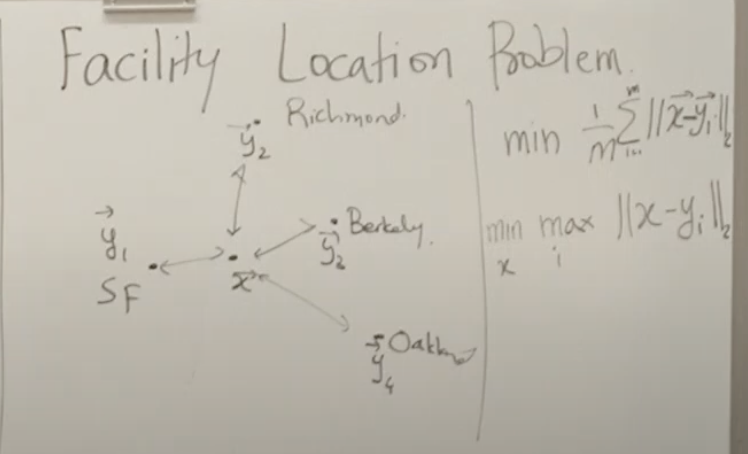
\includegraphics{img/FLP.png}
\end{example}

\begin{example}[Trilateration/GPS]
	A packet is transmitted at $t_i^T$ and received at $t_i^R$ with an offset $\delta$ such that
	\[
t_i^{\text{true}} = t_i^R+\delta
	\]
	\begin{itemize}
		\item Time of flight $f_i = t_i^{\text{true}} - t_i^T = t_i^R+\delta- t_i^T = \Delta_i+\delta$
		\item Distance $cf_i = c \Delta_i+c \delta = \|\v{x}-\v{q}_i\|_2$
	\end{itemize}
	Where c = the speed of light, x is the current location and q is the satellite location. We use 4 satellites, sqare all the equations, and substract them from the equation of satellite \#4.
	\begin{align*}
		\|x-q_4\|_2^2 - \|x-q_1\|_2^2&=x^\top x-x^\top x+0x+const\\
		2(q_4-q)^\top x+2c^2(\Delta_4- \Delta_1)\delta &= c^2(\Delta_1^2- \Delta_4^2)+\|q_4\|_2^2-\|q_1\|_2^2
	\end{align*}
	But what if instead of four satellites, we only have three satellites? We can solve this via SOCP by constructing optimization problem
	\begin{align*}
	&\min \delta\\
	s.t.\;\;\;&2(q_3-q_1)^\top x+2c^2(\Delta_3- \Delta_1)\delta = c^2(\Delta_1^2- \Delta_3^2)+\|q_3\|_2^2-\|q_1\|_2^2\\
	&2(q_3-q_2)^\top x+2c^2(\Delta_3- \Delta_2)\delta = c^2(\Delta_2^2- \Delta_3^2)+\|q_3\|_2^2-\|q_2\|_2^2\\
	&\|x-q_3\|_2=c \Delta_3+c \delta
	\end{align*}
\end{example}

% section second_order_cone_problems (end) \vfill
\section{Newton's Method} % (fold)
\label{sec:newton_s_method}

\begin{remark}
	We call gradient descent a "first-order method" because it works by taking the first-order derivative of the object function. Newton's Method is a "second-order method."
\end{remark}

\begin{definition}
	min f(x). Want $\v{x}_0, \v{x}_1$ converge to $\v{x}$, which is the optimal. Then the Newton step is defined as
	\[
x_{k+1} = x_k-(\nabla^2 f(x_k))^{-1}\nabla f(x_k)
	\]
	Assuming that f is convex and Hessian is PD (so it's invertible).
\end{definition}

\begin{remark}
	For cases where Hessian is PSD, there is a family of method called \textbf{Quasi-Newton methods} which solve the problem using Newton's method approach but pretend the problem is second-order differentiable. It's a simple idea and we should not be intimidated by the jargon.
\end{remark}

\begin{remark}
	Newtons' method does not have a $\eta$. You can do Newton's method by manually plugging in a stepsize but by default the stepsize is always 1.
\end{remark}

\begin{remark}[Pros and Cons of the Newton's method]
	Pros:
	\begin{itemize}
		\item Converge faster than GD
	\end{itemize}

	\noindent Cons:
	\begin{itemize}
		\item You have to do a Hessian inversion everytime, which is computationally expensive.
	\end{itemize}
	\noindent Sometimes it is cheaper to just compute the gradient, but gradient descent also takes more steps. Therefore most of the times it is unclear to us which method is computationally cheaper.
\end{remark}

% section newton_s_method (end)

\end{document}